\chapter{Marco te\'orico}
\label{cap:marco}
En este capítulo se exponen los conceptos teóricos del presente trabajo de tesis. Rellenar al final

\section{Motores de búsqueda verticales}
\label{marco:mbv}
A medida que pasa el tiempo y la Web sigue creciendo, los motores de búsqueda se convierten en una herramienta cada vez más importante para los usuarios. Estas máquinas ayudan a los usuarios a buscar contenido dentro de la Web, puesto que conocen en qué páginas de la Web aparecen qué palabras. Sin un buscador los usuarios estarían obligados a conocer los localizadores de recursos uniformes (URL) de cada uno de los sitios a visitar. Además, los motores de búsquedas en cierto modo conectan la Web, ya que existe un gran número de páginas Web que no tienen referencia desde otras páginas, siendo el único modo de acceder a ellas a través de un motor de búsqueda.

Un motor de búsqueda está construído por diversos componentes, y su arquitectura típica la podemos ver en la Figura \ref{fig:searchenginearchitecture}. Existe un proceso denominado \textit{crawling}, éste posee una tabla con las páginas Web iniciales en las que se extrae el contenido de cada una de ellas. A medida que el \textit{crawler} comienza a encontrar enlaces a otras páginas Web, la tabla de páginas a visitar crece. El contenido que se extrae en el procedimiento de \textit{crawling} es enviado al proceso de indexamiento, este se encarga de crear un índice de las páginas visitadas por el \textit{crawler}. 

\begin{figure}[tp]
\centering
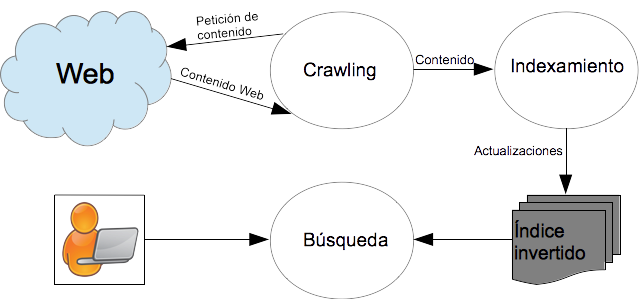
\includegraphics[scale=.75]{images/searchenginearchitecture.png}
\caption{Arquitectura típica de un motor de búsqueda}
\label{fig:searchenginearchitecture}
\end{figure}

Dado el volúmen de datos involucrado en el procesamiento, se debe tener una estructura de datos que permita encontrar cuáles páginas contienen las palabras presentes en la búsqueda, todo esto dentro de un período de tiempo aceptable. El índice invertido es una estructura de datos que contiene una lista con todas las palabras que el proceso de \textit{crawling} ha visto, y asociada a cada palabra se tiene una lista de todas las páginas Web donde ésta palabra aparece mencionada. El motor de búsqueda construye esta estructura con el objetivo de acelerar el proceso de las búsquedas que llegan al sistema. El proceso de búsqueda es el encargado de recibir la consulta (query), generar un \textit{ranking} de las páginas Web que contienen las palabras de la consulta y finalmente generar una respuesta. Las diversas formas de calcular la relevancia de una página Web será explicado en secciones posteriores.

En un motor de búsqueda se pueden encontrar diversos servicios tales como (a) cálculo de las mejores páginas Web para una cierta consulta; (b) construcción de la página Web con los resultados de la consulta; (c) publicidad relacionada con las \textit{queries}; (e) sugerencia de \textit{queries}; entre muchos otros servicios.

Lo que se hace hoy en día es agrupar computadores para procesar una consulta y producir la respuesta de ésta. Este conjunto de computadores recibe el nombre de \textit{cluster}.

La diferencia entre un motor de búsqueda vertical y uno general, es que el primero se centra solo en un contenido específico de la Web. El \textit{crawler} también debe extraer solo el contenido de aquellas páginas Web que están dentro del dominio permitido. Al ser un dominio acotado, las páginas Web a procesar serán menos y por tanto la lista de los términos del índice invertido serán eventualmente de menor tamaño. Sin embargo, en un motor de búsqueda vertical las actualizaciones al índice invertido ocurren con mayor frecuencia.

\section{\'Indice invertido}
\label{marco:ii}
Es una estructura de datos que contiene todos los términos (palabras) encontrados. A cada uno de los términos, está asociado una lista de punteros a los documentos (páginas Web) que contienen dicho término. Además se almacena información que permita realizar el \textit{ranking} de las respuestas a las consultas (queries) que llegan al sistema, por ejemplo, el número de veces que aparece el término en el documento. Esta lista recibe el nombre de lista invertida.

Para construir un índice invertido se debe procesar cada palabra que existe en un documento, registrando su posición y la cantidad de veces que éste se repite. Cuando se procesa el término con la información asociada correspondiente, se almacena en el índice invertido (ver Figura \ref{fig:invertedindex}).

\begin{figure}[tp]
\centering
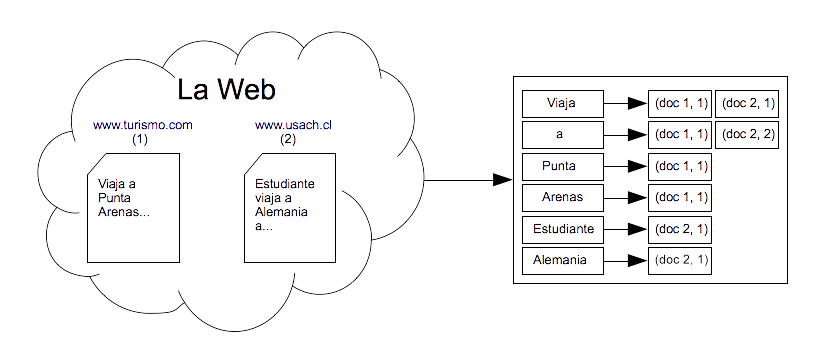
\includegraphics[scale=.75]{images/invertedindex.png}
\caption{\'Indice invertido}
\label{fig:invertedindex}
\end{figure}

El tamaño del índice invertido crece rápido y eventualmente la memoria RAM se agotará antes de procesar toda la colección de documentos. Cuando la memoria RAM se agota, se almacena en disco el índice parcial hasta aquel momento, se libera la memoria y se continúa con el proceso. Además, se debe hacer un \textit{merge} de los índices parciales uniéndo las listas invertidas de cada uno de los términos involucrados.

\section{Estrategias de evaluaci\'on de queries}
\label{marco:eeq}
Existen dos principales estrategias para encontrar los documentos y calcular sus respectivos puntajes de una determinada \textit{query}. Estas son (a) \textit{term-at-a-time} (TAAT) y (b) \textit{document-at-a-time} (DAAT).

\subsection{TAAT}
Este tipo de estrategia procesa los términos de las \textit{queries} uno a uno y acumula el puntaje parcial de los documentos. Las listas invertidas asociadas a un término son procesadas secuencialmente, esto significa que los documentos presente en la lista invertida del término $t_{i}$, obtienen un puntaje parcial antes de comenzar el procesamiento del término $t_{i+1}$. La secuencialidad en este caso es con respecto a los términos contenidos en la \textit{query}.

\subsection{DAAT}
En este tipo de estrategias se valúa la contribución de todos los términos de la query con respecto a un documento antes de evaluar el siguiente documento. Las listas invertidas de cada término de la \textit{query} son procesadas en paralelo, de modo que el puntaje del documento $d_{j}$ se calcula considerando todos los términos de la query al mismo tiempo. Una vez que se obtiene el puntaje del documento $d_{j}$ para la \textit{query} completa, se procede al procesamiento del documento $d_{j+1}$.

\subsection{Consideraciones}
Las estrategias TAAT son mayormente usadas en sistemas de recuperación de información (IR), como son los motores de búsqueda. 
Cuando se tiene un índice invertido pequeño, las estrategias TAAT rinden adecuadamente, sin embargo cuando los índices invertidos son de gran tamaño las estrategias TAAT poseen dos grandes ventajas: (a) Requieren menor cantidad de memoria para su ejecución, ya que el puntaje parcial por documento no necesita ser guardado y (b) Explotan el paralismo de entrada y salida (I/O) más eficientemente procesando las listas invertidas en diferentes discos simultáneamente.


\section{Operaciones sobre listas invertidas}
\label{marco:osli}
Cuando una \textit{query} llega al motor de búsqueda, cada término tiene asociado una lista con todos los documentos en los cuales aparece dicho término. El sistema debe decidir qué documentos se analizarán para obtener la respuesa con el conjunto de los K mejores. 
A continuación se presentan las diferentes formas de operar los documentos pertenecientes a las listas invertidas de una \textit{query}.

\subsection{OR}
\label{marco:or}
Este operador toma las listas invertidas de cada uno de los términos de la \textit{query} y ejecuta la disyunción entre ellas. El resultado de este operador es una lista invertida con todos los documentos que contengan al menos un término de la query. Finalmente, esta lista invertida se ocupará para obtener los mejores K documentos. Un ejemplo sencillo se muestra en la FIGURA \ref{fig:ORoperation}.

\begin{figure}[tp]
\centering
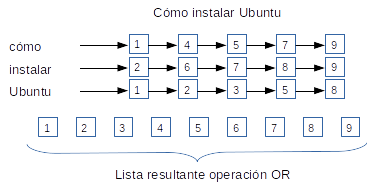
\includegraphics[scale=.75]{images/ORoperation.png}
\caption{Operaci\'on OR}
\label{fig:ORoperation}
\end{figure}

\subsection{AND}
\label{marco:and}
Este operador ejecuta la conjunción entre las listas invertidas de los términos de una \textit{query}. Se obtiene una lista invertida con los documentos que contengan todos los términos de la \textit{query}. Se debe notar que aquí se obtiene una lista resultante de menor que la obtenida en el operador OR (Ver FIGURA \ref{fig:ANDoperation}).

\begin{figure}[tp]
\centering
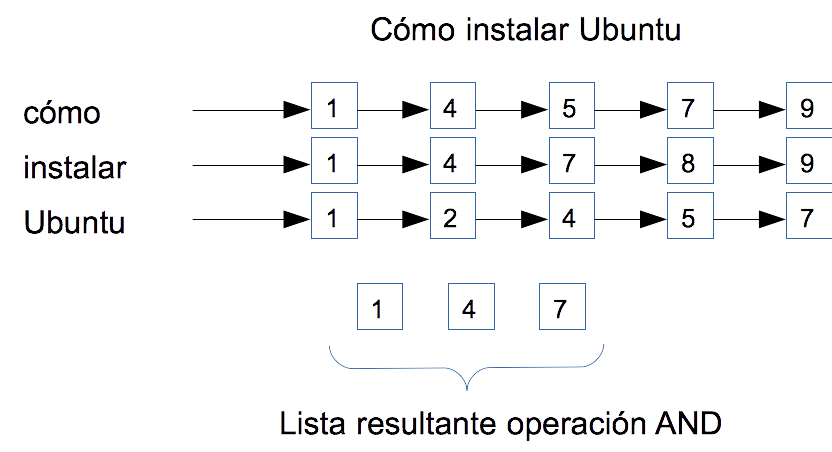
\includegraphics[scale=.75]{images/ANDoperation.png}
\caption{Operaci\'on AND}
\label{fig:ANDoperation}
\end{figure}


\subsection{WAND}
\label{marco:wand}
Método de evaluación de \textit{query} para obtener eficientemente el conjunto de los mejores \textit{top K} documentos que mejor satisfacen la \textit{query} dada. \textit{WAND} \citep{Broder:2003} (\textit{Weak AND}) es un proceso menos estricto que el método \textit{AND} y es basado en dos niveles. Dentro del proceso de evaluación de una \textit{query}, uno de los procesos más costoso en términos de tiempo es el proceso de \textit{scoring}. Este proceso corresponde a entregarle a cada uno de los documentos analizados, un puntaje que representa la relevancia del documento para una \textit{query} dada, esto se denomina evaluación completa o cálculo cálculo del puntaje exacto del documento.

El objetivo de WAND es minimizar la cantidad de evaluaciones completas de los documentos ejecutando un proceso de dos niveles. En el primer nivel se intenta omitir rápidamente grandes porciones de las listas invertida, lo que se traduce en ignorar el cálculo del puntaje exacto de grandes cantidades de documentos, ya que éste cálculo en motores de búsqueda a gran escala es una tarea que requiere de mucho tiempo para llevarse a cabo y depende de factores como la cantidad de ocurrencia del término dentro del documento, el tamaño del documento, entre otros.  

En el primer nivel se itera sobre los documentos del índice invertido de cada término y se identifica candidatos usando una evaluación aproximada. En el segundo nivel, aquellos documentos candidatos son completamente evaluados y su puntaje exacto es calculado. 